% This file was created with tikzplotlib v0.10.1.
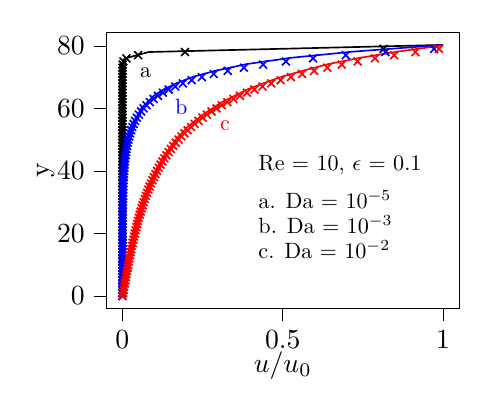
\begin{tikzpicture}
\pgfplotsset{%
    width=0.5\textwidth,
    height=0.42\textwidth
}
\definecolor{darkgray176}{RGB}{176,176,176}

\begin{axis}[
tick align=outside,
tick pos=left,
x grid style={darkgray176},
xlabel={$u/u_0$},
xmin=-0.050203368, xmax=1.050219208,
xtick style={color=black},
y grid style={darkgray176},
ylabel={y},
ymin=-4.1087068, ymax=84.3068908,
ytick style={color=black},
x label style={at={(axis description cs:0.5, -0.12)},anchor=north},
y label style={at={(axis description cs:-0.12,.5)},anchor=south}
]
\addplot [semithick, black, mark=x, mark size=2, mark options={solid}, only marks]
table {%
1.24456663114613e-14 0
1.24456663114613e-14 1
1.24456663114613e-14 2
1.24456663114613e-14 3
1.24456663114613e-14 4
1.24456663114613e-14 5
1.24456663114613e-14 6
1.24456663114613e-14 7
1.24456663114613e-14 8
1.24456663114613e-14 9
1.24456663114613e-14 10
1.24456663114613e-14 11
1.24456663114613e-14 12
1.24456663114613e-14 13
1.24456663114613e-14 14
1.24456663114613e-14 15
1.24456663114613e-14 16
1.24456663114613e-14 17
1.24456663114613e-14 18
1.24456663114613e-14 19
1.24456663114613e-14 20
1.24456663114613e-14 21
1.24456663114613e-14 22
1.24456663114613e-14 23
1.24456663114613e-14 24
1.24456663114613e-14 25
1.24456663114613e-14 26
1.24456663114613e-14 27
1.24456663114613e-14 28
1.24456663114613e-14 29
1.24456663114613e-14 30
1.24456663114613e-14 31
1.24456663114613e-14 32
1.24456663114613e-14 33
1.24456663114613e-14 34
1.24456663114613e-14 35
1.24456663114613e-14 36
9.334249733596e-15 37
1.24456663114613e-14 38
7.77854144466334e-15 39
1.24456663114613e-14 40
1.24456663114613e-14 41
2.02242077561247e-14 42
2.48913326229227e-14 43
2.48913326229227e-14 44
2.333562433399e-14 45
2.48913326229227e-14 46
2.02242077561247e-14 47
1.4001374600394e-14 48
1.55570828893267e-14 49
1.55570828893267e-14 50
1.55570828893267e-14 51
1.52999953448103e-14 52
1.58184927459258e-14 53
1.62420713749098e-14 54
1.59370484186994e-14 55
2.32865968295828e-14 56
6.96670575078039e-14 57
2.53329791365623e-13 58
9.77585936724286e-13 59
3.84754203717842e-12 60
1.51360109883514e-11 61
5.94511347499375e-11 62
2.33546818105755e-10 63
9.17551563386863e-10 64
3.60484498365391e-09 65
1.41625610156146e-08 66
5.56412183840858e-08 67
2.18600623534938e-07 68
8.58827980169011e-07 69
3.3741240854711e-06 70
1.32561139264114e-05 71
5.20801996055482e-05 72
0.000204613321431925 73
0.000803922601503561 74
0.00315914463838044 75
0.0124228019131766 76
0.048981649066456 77
0.195213477968454 78
0.814486339914766 79
};
\addplot [semithick, blue, mark=x, mark size=2, mark options={solid}, only marks]
table {%
4.31252904233955e-06 0
1.30043756758872e-05 1
2.18976233284463e-05 2
3.11300047403877e-05 3
4.08445050359419e-05 4
5.11915752333114e-05 5
6.23314615767758e-05 6
7.44366868643258e-05 7
8.7694722131965e-05 8
0.000102310890327055 9
0.000118511546886296 10
0.000136547586744953 11
0.000156698332253197 12
0.000179275862457426 13
0.000204629851197558 14
0.000233152989396351 15
0.000265287076073961 16
0.000301529873254798 17
0.000342442831944973 18
0.000388659810077859 19
0.000440896919182237 20
0.000499963654474145 21
0.000566775483483918 22
0.000642368091894172 23
0.000727913511791193 24
0.000824738388234659 25
0.000934344674690691 26
0.00105843308787736 27
0.001198929698006 28
0.001358016082782 29
0.00153816353336028 30
0.00174217186914992 31
0.00197321349771788 32
0.00223488344726883 33
0.00253125620424523 34
0.00286695031095622 35
0.00324720181925726 36
0.00367794786101411 37
0.00416592178794492 38
0.00471876155790746 39
0.00534513330843777 40
0.00605487236867916 41
0.00685914432810811 42
0.00777062921640536 43
0.00880373236850245 44
0.00997482617128446 45
0.0113025276373734 46
0.0128080176566601 47
0.0145154088763646 48
0.016452170503842 49
0.0186496199758299 50
0.0211434934740277 51
0.0239746097947186 52
0.027189645235821 53
0.0308420411273957 54
0.0349930706374738 55
0.0397130978470005 56
0.0450830702241144 57
0.0511962961008863 58
0.0581605723269017 59
0.0661007449815682 60
0.0751618092997829 61
0.0855126857852895 62
0.0973508506266284 63
0.110908053913335 64
0.126457434375988 65
0.144322442530345 66
0.164888127012573 67
0.188615539038421 68
0.216060293539266 69
0.247896732548432 70
0.284949728556041 71
0.328237039861366 72
0.379026441809053 73
0.438913860974206 74
0.509931857396559 75
0.594702756653464 76
0.696658798498429 77
0.82036513410246 78
0.972004642878822 79
};
\addplot [semithick, red, mark=x, mark size=2, mark options={solid}, only marks]
table {%
0.000840807730202179 0
0.00252374002891129 1
0.00421064514169528 2
0.00590422301560292 3
0.00760722406399993 4
0.0093224541292452 5
0.0110527798043359 6
0.0128011341334493 7
0.0145705227142618 8
0.0163640302274629 9
0.0181848274224858 10
0.0200361785915075 11
0.0219214495677422 12
0.0238441162879488 13
0.02580777396379 14
0.0278161469113447 15
0.0298730990936372 16
0.0319826454370256 17
0.03414896398883 18
0.0363764089909919 19
0.0386695249526958 20
0.0410330618139198 21
0.0434719913020115 22
0.045991524594769 23
0.048597131415957 24
0.0512945607035784 25
0.0540898630069749 26
0.0569894147867491 27
0.0599999448116496 28
0.0631285628693659 29
0.0663827910336169 30
0.0697705977592879 31
0.0733004351100023 32
0.0769812794601732 33
0.0808226760559616 34
0.0848347878681447 35
0.0890284492251602 36
0.093415224778052 37
0.0980074744213649 38
0.10281842487749 39
0.107862248747575 40
0.11315415194259 41
0.118710470535516 42
0.124548778223299 43
0.130688005758087 44
0.13714857390646 45
0.143952541726836 46
0.151123772226252 47
0.158688117774344 48
0.16667362802463 49
0.175110783530834 50
0.184032758762945 51
0.193475718838814 52
0.203479155013078 53
0.214086264828765 54
0.225344383868796 55
0.237305477279936 56
0.250026700727124 57
0.263571042227651 58
0.27800805848274 59
0.293414721958907 60
0.309876398184924 61
0.327487976665617 62
0.346355183654158 63
0.366596111002916 64
0.38834300273305 65
0.411744350214126 66
0.436967358439494 67
0.46420086048894 68
0.493658775772297 69
0.52558423122014 70
0.560254494803828 71
0.597986909745764 72
0.639146068402652 73
0.68415253101462 74
0.7334934817619 75
0.787735830456516 76
0.847542423415742 77
0.913692236825843 78
0.987105712072561 79
};
\addplot [semithick, black]
table {%
0.0012891 -0.089536
-0.00018416 7.854
-0.00018416 15.948
-0.00018416 23.8912
0.0012891 31.9856
-0.00018416 36.032
-0.00018416 37.9808
-0.00018416 39.9288
-0.00018416 41.8776
-0.00018416 47.8728
-0.00018416 55.9664
-0.00018416 63.9104
-0.00018416 72.004
-0.00018416 73.952
0.005709 75.9016
0.08232 78.0144
1.0002 80.288
};
\addplot [semithick, blue]
table {%
-0.00018416 -0.089816
-0.00018416 8.004
-0.00018416 15.948
-0.00018416 23.8912
-0.00018416 31.9848
0.0027624 37.8312
0.005709 39.9304
0.0071823 41.8784
0.013076 47.8752
0.027808 53.8736
0.058748 60.024
0.098527 64.0784
0.12799 66.0328
0.16777 67.9888
0.22081 70.0968
0.29153 72.0584
0.38877 74.1752
0.52431 76.1488
0.71878 78.1336
1.0002 80.288
};
\addplot [semithick, red]
table {%
-0.00018416 -0.089816
0.013076 7.85648
0.027808 15.9528
0.045488 23.9
0.069061 31.9984
0.076427 33.948
0.085267 36.048
0.094107 37.9984
0.10295 39.948
0.11326 41.8984
0.12357 43.9992
0.1663 50.0024
0.20313 54.056
0.25028 57.9616
0.31068 62.02
0.39024 66.0816
0.44033 68.0392
0.49779 70.1488
0.56556 72.1096
0.64512 74.2232
0.74236 76.1896
0.85875 78.16
1.0002 80.136
};
\draw (axis cs:0.4,40) node[
  scale=0.8,
  anchor=base west,
  text=black,
  rotate=0.0
]{Re = 10, $\epsilon$ = 0.1};
\draw (axis cs:0.4,28) node[
  scale=0.8,
  anchor=base west,
  text=black,
  rotate=0.0
]{a. Da = ${10^{-5}}$};
\draw (axis cs:0.4,20) node[
  scale=0.8,
  anchor=base west,
  text=black,
  rotate=0.0
]{b. Da = ${10^{-3}}$};
\draw (axis cs:0.4,12) node[
  scale=0.8,
  anchor=base west,
  text=black,
  rotate=0.0
]{c. Da = ${10^{-2}}$};
\draw (axis cs:0.03,70) node[
  scale=0.8,
  anchor=base west,
  text=black,
  rotate=0.0
]{a};
\draw (axis cs:0.14,58) node[
  scale=0.8,
  anchor=base west,
  text=blue,
  rotate=0.0
]{b};
\draw (axis cs:0.28,53) node[
  scale=0.8,
  anchor=base west,
  text=red,
  rotate=0.0
]{c};
\end{axis}

\end{tikzpicture}